\chapter{Inventory Policy from Forecasts}

\begin{weekbox}
\textbf{Theme.} Predict-then-optimise in its purest form: the forecast sets the expected need, the forecast
\emph{error} sets the buffer, and the cost of each error sets how big the buffer should be.\\
\textbf{Outcomes.} LO5, LO1.\quad \textbf{Tools.} NumPy, SciPy, pandas.\\
\textbf{Data.} Mboa rice and bread (S1); the Week 3 forecasts and errors for 157 real items; a simulated four-stage
supply chain.\\
\textbf{Lab.} EOQ and its flat cost curve; safety stock from forecast error; $(s,Q)$ and $(R,S)$ policies tested by
simulation; the newsvendor with a forecast quantile; the bullwhip effect.\\
\textbf{Deliverable.} Lab notebook. \textbf{CA2} (forecast and stock policy) follows this week.
\end{weekbox}

\begin{timetable}
0:00--0:20 & Briefing & ``We had 18 days of stock on average and still ran out of rice in December.''\\
0:20--1:10 & Concepts & Inventory costs, service measures, EOQ, safety stock, review policies, newsvendor, bullwhip\\
1:10--2:40 & Guided lab & Lab 4, Steps 1--5 (break at 1:55)\\
2:40--3:40 & Challenge & Exercises 4.3--4.8\\
3:40--4:00 & Debrief & What service level would you set for bread, and what does it cost per year?\\
\end{timetable}

\section{Why hold stock, and what it costs}
Stock decouples supply from demand: it lets a store order in economical batches (\emph{cycle stock}), protects against
forecast errors during the lead time (\emph{safety stock}), and covers goods on their way (\emph{pipeline stock}). Each
costs money:
\begin{itemize}[nosep]
\item \textbf{ordering cost} $K$ per order: transport, handling, administration;
\item \textbf{holding cost} $h$ per unit per year: capital (often 15--25\% of value in Cameroon at current lending
rates), space, insurance, spoilage and obsolescence;
\item \textbf{shortage cost}: lost margin, lost future business, emergency supply. The hardest to measure and the one
that decides the service level.
\end{itemize}

\begin{definition}{Two service measures}
\emph{Cycle service level} (CSL, ``$\alpha$'') is the probability of \emph{no} stock-out in a replenishment cycle.
\emph{Fill rate} (``$\beta$'') is the fraction of demand served from stock. They are not the same: with large orders,
cycles are rare and short stock-outs lose few units, so a 90\% CSL can mean a 99\% fill rate. Customers feel the fill
rate; textbooks often compute the CSL. Say which one you mean.
\end{definition}

\section{How much to order: EOQ}
With steady annual demand $D$, the annual cost of ordering $Q$ units at a time is
$TC(Q)=\frac{D}{Q}K+\frac{Q}{2}h$.
\begin{keyformula}{Economic order quantity}
\[ Q^*=\sqrt{\frac{2DK}{h}},\qquad TC(Q^*)=\sqrt{2DKh},\qquad \frac{TC(Q)}{TC(Q^*)}=\frac12\left(\frac{Q}{Q^*}+\frac{Q^*}{Q}\right). \]
\end{keyformula}
The last expression is the reason EOQ survives in practice: the cost curve is flat. Ordering 25\% more or less than
$Q^*$ raises cost by only 2.5\%, so $Q^*$ can be rounded to pallets, truckloads or a weekly rhythm at almost no cost.

\section{When to order: reorder point and safety stock}
In a continuous-review $(s,Q)$ policy, an order of $Q$ is placed when the inventory position (on hand + on order $-$
backorders) falls to the reorder point $s$. The order arrives after lead time $L$. Stock runs out if demand during $L$
exceeds $s$.

\begin{figure}[H]
\centering
\begin{tikzpicture}[x=0.38cm,y=0.042cm]
  \draw[-{Latex},slate] (0,0)--(33,0) node[right,font=\sffamily\scriptsize]{time};
  \draw[-{Latex},slate] (0,0)--(0,125) node[above,font=\sffamily\scriptsize]{stock};
  \fill[orange!12] (0,0) rectangle (32,22);
  \draw[orange,dashed] (0,22)--(32,22) node[right,font=\sffamily\scriptsize]{safety stock};
  \draw[brick,dashed] (0,52)--(32,52) node[right,font=\sffamily\scriptsize]{reorder point $s$};
  \draw[navy,thick] (0,110)--(8,52)--(11,30)--(11,110)--(19,52)--(22,22)--(22,102)--(29,52)--(32,40);
  \draw[{Latex}-{Latex},teal] (8,62)--(11,62) node[midway,above,font=\sffamily\scriptsize]{$L$};
  \draw[{Latex}-{Latex},teal] (19,62)--(22,62) node[midway,above,font=\sffamily\scriptsize]{$L$};
  \draw[{Latex}-{Latex},slate] (11.6,30)--(11.6,110) node[midway,right,font=\sffamily\scriptsize]{$Q$};
\end{tikzpicture}
\caption{The $(s,Q)$ sawtooth. Cycle stock is $Q/2$ on average; safety stock is what is left when an order arrives,
on average.}
\end{figure}

\begin{keyformula}{Reorder point from forecast error}
\[ s=\hat D_L + z_\alpha\,\sigma_L,\qquad \text{safety stock}=z_\alpha\,\sigma_L, \]
where $\hat D_L$ is the forecast of demand over the lead time, $\sigma_L$ is the standard deviation of the
\emph{lead-time forecast error}, and $z_\alpha=\Phi^{-1}(\alpha)$ for a target CSL $\alpha$. Under independence
$\sigma_L\approx\sigma_1\sqrt L$; with random lead time,
$\sigma_L=\sqrt{\bar L\,\sigma_1^2+\bar d^{\,2}\sigma_{\text{LT}}^2}$.
\end{keyformula}

The textbook formula uses the standard deviation of \emph{demand}. That is right only when the forecast is a constant
mean. When the forecast follows trend and season, the uncertainty that remains is the forecast error, which is
smaller; buffering against the predictable part of demand wastes money. This is the precise link between Week 3 and
Week 4: \textbf{a better forecast is worth exactly the safety stock it removes}.

\begin{example}{Safety stock and the value of a better forecast}
Rice at S1: lead time $L=7$ days, unit cost 2\,800\xaf, holding 25\% a year. For CSL 95\%, $z=1.645$. Using the standard
deviation of lead-time demand, $\sigma_L=26.6$, gives $1.645\times26.6=44$ units. Using the lead-time forecast error,
$\sigma_L=20.8$, gives 34 units. The 10 units saved are worth $10\times700=7\,000$\xaf\ a year for one item in one store;
across 72 store--items and a better forecast the saving runs to several million francs, with the same service.
\end{example}

\paragraph{Periodic review $(R,S)$} Many stores order on fixed days. Every $R$ periods, order up to $S$:
$S=\hat D_{R+L}+z_\alpha\sigma_{R+L}$. The protection interval is $R+L$, not $L$, because an order must cover until the
\emph{next} order arrives. Periodic review needs more safety stock but allows joint orders and fixed delivery rounds.

\section{One chance to order: the newsvendor}
Bread, newspapers, fresh fish, seasonal fashion: you order once, demand $D$ is uncertain, and leftovers lose value.
Let $c_u$ be the cost of one unit too few (lost margin, $p-c$) and $c_o$ the cost of one unit too many (cost minus
salvage, $c-v$).
\begin{keyformula}{Newsvendor critical ratio}
\[ F(Q^*)=\frac{c_u}{c_u+c_o}\quad\Longrightarrow\quad Q^*=F^{-1}\!\left(\frac{c_u}{c_u+c_o}\right). \]
The optimal order is a \emph{quantile} of the demand forecast distribution, not its mean.
\end{keyformula}
If the margin is thin and waste is costly, the critical ratio is below 0.5 and the optimal order is \emph{below} the
expected demand: running out of bread on most days is the profit-maximising policy. If the margin is wide, order
above the mean. This is why Week 3 insisted on quantile forecasts.

\begin{realcase}{Sport Obermeyer}
The US skiwear maker had to commit to production months before the season. Fisher, Hammond, Obolensky and Raman
(\emph{Harvard Business Review}, 1994) describe how it asked a panel of managers for independent forecasts, used their
disagreement as a measure of uncertainty, and committed early production to the predictable styles while keeping
flexible capacity for the uncertain ones. The newsvendor logic, applied style by style, reportedly cut the cost of
stock-outs and markdowns substantially.
\end{realcase}

\section{The bullwhip effect}
Order variability grows as it moves up a supply chain, from retailer to wholesaler to distributor to factory, even
when consumer demand is steady.
\begin{definition}{Bullwhip effect}
The amplification of order variance relative to demand variance at each upstream stage of a supply chain:
$\mathrm{BW}=\mathrm{Var}(\text{orders})/\mathrm{Var}(\text{demand})>1$.
\end{definition}
Lee, Padmanabhan and Whang (\emph{Sloan Management Review}, 1997) named four causes: (1) each stage forecasts from the
orders it receives rather than from end demand; (2) order batching; (3) price promotions that encourage forward
buying; (4) rationing and shortage gaming. For a stage using an order-up-to policy with a moving-average forecast over
$m$ periods and lead time $L$, Chen et al.\ (2000) show
\[ \frac{\mathrm{Var}(q)}{\mathrm{Var}(D)}\ \ge\ 1+\frac{2L}{m}+\frac{2L^2}{m^2}. \]
Cures follow from the causes: share point-of-sale data upstream, shorten lead times, smooth orders, use everyday low
prices, and allocate scarce stock by past sales rather than by orders.

\begin{realcase}{Procter \& Gamble and Pampers}
P\&G found that orders from distributors for Pampers nappies varied far more than nappy consumption, which is about
as steady as demand gets, and that its own orders to suppliers varied more still. It was the example that opened Lee,
Padmanabhan and Whang's article and led to vendor-managed inventory with retailers sharing sales data.
\end{realcase}

% ------------------------------------------------------------------ LAB
\section{Practical Lab 4: From forecasts to stock policies}
\begin{labbox}{Practical lab --- inventory policies tested by simulation}
\textbf{Goal.} Size orders and buffers from forecasts and their errors, then test every policy by simulating it on
demand it has not seen. \textbf{Files.} \texttt{data/sales.csv}, \texttt{data/products.csv},
\texttt{real/weekly\_cv\_forecasts.parquet} (Lab 3). \textbf{Time.} 90 minutes.
\end{labbox}

\step{Step 1: EOQ and the flat cost curve}
\codeout{lab4_s1}{EOQ for 5\,kg rice at Yaoundé Centre.}
\interp{The EOQ is 560 bags, about four weeks of demand. Ordering anywhere between 0.8 and 1.25 times that costs
only 2.5\% more, so the store can order ``one truck every four weeks'' or even every three without worrying.}

\step{Step 2: Safety stock from forecast error, tested on 2024}
\codeout{lab4_s2}{Three ways to measure uncertainty, and an $(s,Q)$ simulation with backorders.}
\interp{The lead-time forecast error ($\sigma=20.8$) is smaller than the unconditional variability of lead-time
demand (26.6), so the error-based buffer is 10 units smaller. The simulation shows a second, less obvious lesson.
With EOQ batches the store reorders only 15 times a year, so even without safety stock the fill rate is 99.1\%: big
orders buffer by themselves, at a cost in average stock. With weekly orders (perhaps forced by back-room space),
the fill rate without safety stock falls to 94.2\%, and the error-based buffer restores it to 99.7\% for
23\,000\xaf\ a year. Safety stock matters most when orders are small and frequent.}

\step{Step 3: Newsvendor for bread}
\codeout{lab4_s3}{Ordering bread at the critical-ratio quantile of the forecast, simulated over 2024.}
\interp{With 60\xaf\ margin and 150\xaf\ lost on every unsold loaf, the critical ratio is 0.29: order about 18\% below the
forecast. That plan earns 1.37\,M\xaf\ in 2024 against 1.17\,M\xaf\ for ordering the forecast, a gain of 16\%, while
waste falls from 4\,718 to 1\,929 loaves. Bread is out of stock on two days in three; that is the price of the
thin margin. A manager who finds that unacceptable should change the economics (raise price, find a better
outlet for day-old bread), and the critical ratio will tell how much service each change buys.}

\begin{pitfall}{A lucky benchmark}
The fixed ``2023 average'' order looks good (1.29\,M\xaf) only by accident: demand grew in 2024, which pushed a
fixed order below the mean, close to where the critical ratio wants it. In a shrinking year the same rule would
lose money. Judge a policy by its logic and test it on more than one period.
\end{pitfall}

\step{Step 4: Periodic review on real items and real errors}
\codeout{lab4_s4}{An $(R,S)$ policy for 157 items: errors measured April--July, policy run August--November 2011.}
\interp{At every target the achieved fill rate is lower than a fill rate usually is for that CSL (fill rate normally
exceeds CSL). The reason is Lab 3's warning: errors measured in calm summer months understate autumn errors, and the
forecast under-shoots the peak by 4\%. Moving from a 95\% to a 99\% target buys 2.3 points of fill rate for 26\% more
stock. In practice, re-estimate $\sigma$ before the peak or use a seasonal error model.}

\step{Step 5: The bullwhip effect}
\codeout{lab4_s5}{A four-stage chain, each stage ordering up to $(L+1)$ times its moving-average forecast.}
\begin{figure}[H]\centering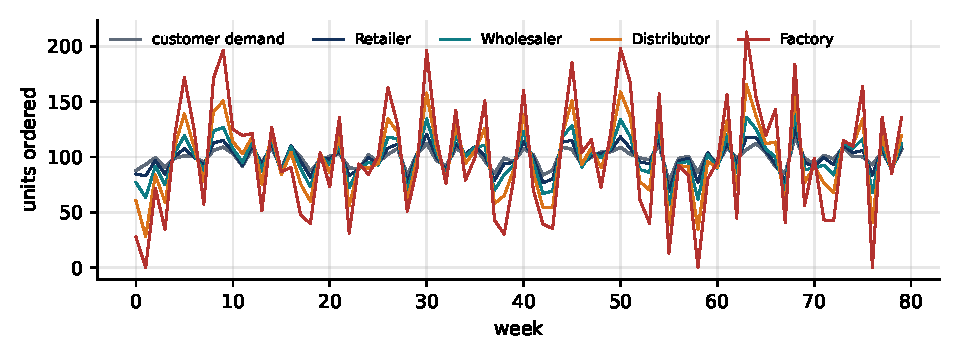
\includegraphics[width=0.92\linewidth]{../figs/lab4_bullwhip.pdf}
\caption{Steady customer demand (grey) and orders at each upstream stage when every stage forecasts from incoming orders.}\end{figure}
\interp{Customer demand has a CV of 10\%, yet the factory sees orders 37 times as variable. Each stage amplifies by
about 2.2--2.6, a little above the theoretical lower bound of 1.62 because orders cannot be negative. When every
stage forecasts from end-customer sales (shared POS data), the factory's amplification falls from 37 to 10. Nothing
else changed: same policies, same lead times. Information sharing is worth more than a better forecasting model.}

\paragraph{So what (model answer)} \emph{Bread should be ordered at about 82\% of the forecast: it raises annual profit
at Yaoundé Centre by about 190\,000\xaf\ and cuts waste by 60\%. Safety stock for staples should be set from forecast
errors, not demand variability, and re-estimated before December. Sharing store sales with our suppliers would
reduce the order swings that cause their late deliveries.}

% ------------------------------------------------------------------ EXERCISES
\section{Exercises}
\begin{enumerate}[label=\textbf{4.\arabic*},leftmargin=2.4em]
\item \emph{(EOQ)} Cooking oil: $D=11\,000$ bottles a year, $K=15\,000$\xaf, unit cost 1\,100\xaf, holding 25\%. Compute
$Q^*$ and $TC^*$. The supplier offers 2\% off for orders of at least 2\,000 bottles. Should Mboa accept?
\item \emph{(Service measures)} Explain with a numerical example why a 90\% CSL can coexist with a 99\% fill rate.
\item \emph{(Safety stock)} Daily forecast error sd is 6 units, lead time 9 days with sd 2 days, mean demand 40 a day.
Compute $\sigma_L$ and the safety stock for 97.5\% CSL. Which source of uncertainty dominates, and what would you
negotiate with the supplier?
\item \emph{(Newsvendor)} A trader buys fresh fish at 1\,500\xaf/kg, sells at 2\,400\xaf/kg, and sells leftovers to a
smoker at 900\xaf/kg. Daily demand is normal with mean 80\,kg, sd 20\,kg. Find the optimal purchase and expected
leftovers. How does the answer change if leftovers must be thrown away?
\item \emph{(Simulation)} Modify Step 2 so that lead time is random (5--9 days uniformly). How much extra safety stock
keeps the weekly-order fill rate at 99\%?
\item \emph{(Real data)} In Step 4, estimate $\sigma$ separately by XYZ class and set the target CSL by ABC class (A
98\%, B 95\%). Report fill rate and stock by class.
\item \emph{(Bullwhip)} In Step 5, set the lead time to 1 and then 4. Plot the factory's amplification against $L$ and
compare with the bound.
\item \emph{(Judgement)} The Bafoussam manager wants a 99.5\% CSL ``for everything''. Write a reply, with numbers from
this week, explaining what that would cost and proposing an alternative.
\end{enumerate}

\section{Take-home assignment 4}
For ten Mboa store--product series of your choice: forecast (Week 3 methods), set a policy (EOQ-based $(s,Q)$ or weekly
$(R,S)$, with error-based safety stock), simulate it on 2024, and report fill rate, average stock value and annual
cost. Compare with the store's current rule ``order two weeks of last month's average every Monday''.
